%%
% Copyright (c) 2017 - 2020, Pascal Wagler;
% Copyright (c) 2014 - 2020, John MacFarlane
%
% All rights reserved.
%
% Redistribution and use in source and binary forms, with or without
% modification, are permitted provided that the following conditions
% are met:
%
% - Redistributions of source code must retain the above copyright
% notice, this list of conditions and the following disclaimer.
%
% - Redistributions in binary form must reproduce the above copyright
% notice, this list of conditions and the following disclaimer in the
% documentation and/or other materials provided with the distribution.
%
% - Neither the name of John MacFarlane nor the names of other
% contributors may be used to endorse or promote products derived
% from this software without specific prior written permission.
%
% THIS SOFTWARE IS PROVIDED BY THE COPYRIGHT HOLDERS AND CONTRIBUTORS
% "AS IS" AND ANY EXPRESS OR IMPLIED WARRANTIES, INCLUDING, BUT NOT
% LIMITED TO, THE IMPLIED WARRANTIES OF MERCHANTABILITY AND FITNESS
% FOR A PARTICULAR PURPOSE ARE DISCLAIMED. IN NO EVENT SHALL THE
% COPYRIGHT OWNER OR CONTRIBUTORS BE LIABLE FOR ANY DIRECT, INDIRECT,
% INCIDENTAL, SPECIAL, EXEMPLARY, OR CONSEQUENTIAL DAMAGES (INCLUDING,
% BUT NOT LIMITED TO, PROCUREMENT OF SUBSTITUTE GOODS OR SERVICES;
% LOSS OF USE, DATA, OR PROFITS; OR BUSINESS INTERRUPTION) HOWEVER
% CAUSED AND ON ANY THEORY OF LIABILITY, WHETHER IN CONTRACT, STRICT
% LIABILITY, OR TORT (INCLUDING NEGLIGENCE OR OTHERWISE) ARISING IN
% ANY WAY OUT OF THE USE OF THIS SOFTWARE, EVEN IF ADVISED OF THE
% POSSIBILITY OF SUCH DAMAGE.
%%

%%
% This is the Eisvogel pandoc LaTeX template.
%
% For usage information and examples visit the official GitHub page:
% https://github.com/Wandmalfarbe/pandoc-latex-template
%%

% Options for packages loaded elsewhere
\PassOptionsToPackage{unicode}{hyperref}
\PassOptionsToPackage{hyphens}{url}
\PassOptionsToPackage{dvipsnames,svgnames*,x11names*,table}{xcolor}
%
\documentclass[
  14pt
  american,
  paper=a4,
  ,captions=tableheading
]{scrreprt}
\usepackage{amsmath,amssymb}
\usepackage{lmodern}
\usepackage{setspace}
\setstretch{1.2}
\usepackage{amsmath}
\usepackage{ifxetex,ifluatex}
\ifnum 0\ifxetex 1\fi\ifluatex 1\fi=0 % if pdftex
  \usepackage[T1]{fontenc}
  \usepackage[utf8]{inputenc}
  \usepackage{textcomp} % provide euro and other symbols
  \usepackage{amssymb}
\else % if luatex or xetex
  \usepackage{unicode-math}
  \defaultfontfeatures{Scale=MatchLowercase}
  \defaultfontfeatures[\rmfamily]{Ligatures=TeX,Scale=1}
  \setmainfont[]{DejaVu Sans}
  \setmonofont[]{Source Code Pro}
\fi
% Use upquote if available, for straight quotes in verbatim environments
\IfFileExists{upquote.sty}{\usepackage{upquote}}{}
\IfFileExists{microtype.sty}{% use microtype if available
  \usepackage[]{microtype}
  \UseMicrotypeSet[protrusion]{basicmath} % disable protrusion for tt fonts
}{}
\makeatletter
\@ifundefined{KOMAClassName}{% if non-KOMA class
  \IfFileExists{parskip.sty}{%
    \usepackage{parskip}
  }{% else
    \setlength{\parindent}{0pt}
    \setlength{\parskip}{6pt plus 2pt minus 1pt}}
}{% if KOMA class
  \KOMAoptions{parskip=half}}
\makeatother
\usepackage{xcolor}
\definecolor{default-linkcolor}{HTML}{A50000}
\definecolor{default-filecolor}{HTML}{A50000}
\definecolor{default-citecolor}{HTML}{4077C0}
\definecolor{default-urlcolor}{HTML}{4077C0}
\IfFileExists{xurl.sty}{\usepackage{xurl}}{} % add URL line breaks if available
\IfFileExists{bookmark.sty}{\usepackage{bookmark}}{\usepackage{hyperref}}
\hypersetup{
  pdftitle={Books.jl},
  pdfauthor={Rik Huijzer},
  pdflang={en-US},
  hidelinks,
  breaklinks=true,
  pdfcreator={LaTeX via pandoc with the Eisvogel template}}
\urlstyle{same} % disable monospaced font for URLs
\usepackage[top=20mm,left=24mm,right=24mm,bottom=28mm]{geometry}
\usepackage{listings}
\newcommand{\passthrough}[1]{#1}
\lstset{defaultdialect=[5.3]Lua}
\lstset{defaultdialect=[x86masm]Assembler}
\usepackage{longtable,booktabs,array}
\usepackage{calc} % for calculating minipage widths
% Correct order of tables after \paragraph or \subparagraph
\usepackage{etoolbox}
\makeatletter
\patchcmd\longtable{\par}{\if@noskipsec\mbox{}\fi\par}{}{}
\makeatother
% Allow footnotes in longtable head/foot
\IfFileExists{footnotehyper.sty}{\usepackage{footnotehyper}}{\usepackage{footnote}}
\makesavenoteenv{longtable}
% add backlinks to footnote references, cf. https://tex.stackexchange.com/questions/302266/make-footnote-clickable-both-ways
\usepackage{footnotebackref}
\usepackage{graphicx}
\makeatletter
\def\maxwidth{\ifdim\Gin@nat@width>\linewidth\linewidth\else\Gin@nat@width\fi}
\def\maxheight{\ifdim\Gin@nat@height>\textheight\textheight\else\Gin@nat@height\fi}
\makeatother
% Scale images if necessary, so that they will not overflow the page
% margins by default, and it is still possible to overwrite the defaults
% using explicit options in \includegraphics[width, height, ...]{}
\setkeys{Gin}{width=\maxwidth,height=\maxheight,keepaspectratio}
% Set default figure placement to htbp
\makeatletter
\def\fps@figure{htbp}
\makeatother
\setlength{\emergencystretch}{3em} % prevent overfull lines
\providecommand{\tightlist}{%
  \setlength{\itemsep}{0pt}\setlength{\parskip}{0pt}}
\setcounter{secnumdepth}{5}

% Make use of float-package and set default placement for figures to H.
% The option H means 'PUT IT HERE' (as  opposed to the standard h option which means 'You may put it here if you like').
\usepackage{float}
\floatplacement{figure}{H}

\makeatletter
\@ifpackageloaded{subfig}{}{\usepackage{subfig}}
\@ifpackageloaded{caption}{}{\usepackage{caption}}
\captionsetup[subfloat]{margin=0.5em}
\AtBeginDocument{%
\renewcommand*\figurename{Figure}
\renewcommand*\tablename{Table}
}
\AtBeginDocument{%
\renewcommand*\listfigurename{List of Figures}
\renewcommand*\listtablename{List of Tables}
}
\@ifpackageloaded{float}{}{\usepackage{float}}
\floatstyle{ruled}
\@ifundefined{c@chapter}{\newfloat{codelisting}{h}{lop}}{\newfloat{codelisting}{h}{lop}[chapter]}
\floatname{codelisting}{Listing}
\newcommand*\listoflistings{\listof{codelisting}{List of Listings}}
\makeatother
\ifxetex
      % Load polyglossia as late as possible: uses bidi with RTL langages (e.g. Hebrew, Arabic)
  \usepackage{polyglossia}
  \setmainlanguage[variant=american]{english}
\else
  \usepackage[main=american]{babel}
% get rid of language-specific shorthands (see #6817):
\let\LanguageShortHands\languageshorthands
\def\languageshorthands#1{}
\fi
\ifluatex
  \usepackage{selnolig}  % disable illegal ligatures
\fi
\newlength{\cslhangindent}
\setlength{\cslhangindent}{1.5em}
\newenvironment{cslreferences}%
  {\setlength{\parindent}{0pt}%
  \everypar{\setlength{\hangindent}{\cslhangindent}}\ignorespaces}%
  {\par}

\title{Books.jl}
\usepackage{etoolbox}
\makeatletter
\providecommand{\subtitle}[1]{% add subtitle to \maketitle
  \apptocmd{\@title}{\par {\large #1 \par}}{}{}
}
\makeatother
\subtitle{Create books with Julia}
\author{Rik Huijzer}
\date{}



%%
%% added
%%

%
% language specification
%
% If no language is specified, use English as the default main document language.
%



%
% for the background color of the title page
%
\usepackage{pagecolor}
\usepackage{afterpage}

%
% break urls
%
\PassOptionsToPackage{hyphens}{url}

%
% When using babel or polyglossia with biblatex, loading csquotes is recommended
% to ensure that quoted texts are typeset according to the rules of your main language.
%
\usepackage{csquotes}

%
% captions
%
\definecolor{caption-color}{HTML}{777777}
\usepackage[font={stretch=1.2}, textfont={color=caption-color}, position=top, skip=4mm, labelfont=bf, singlelinecheck=false, justification=raggedright]{caption}

%
% blockquote
%
\definecolor{blockquote-border}{RGB}{221,221,221}
\definecolor{blockquote-text}{RGB}{119,119,119}
\usepackage{mdframed}
\newmdenv[rightline=false,bottomline=false,topline=false,linewidth=3pt,linecolor=blockquote-border,skipabove=\parskip]{customblockquote}
\renewenvironment{quote}{\begin{customblockquote}\list{}{\rightmargin=0em\leftmargin=0em}%
\item\relax\color{blockquote-text}\ignorespaces}{\unskip\unskip\endlist\end{customblockquote}}

%
% Source Sans Pro as the de­fault font fam­ily
% Source Code Pro for monospace text
%
% 'default' option sets the default
% font family to Source Sans Pro, not \sfdefault.
%

\ifnum 0\ifxetex 1\fi\ifluatex 1\fi=0 % if pdftex
    \else % if not pdftex
    \fi

%
% heading color
%
\definecolor{heading-color}{RGB}{40,40,40}
% \addtokomafont{section}{\color{heading-color}}
% When using the classes report, scrreprt, book,
% scrbook or memoir, uncomment the following line.
% \addtokomafont{chapter}{\color{heading-color}}

%
% variables for title, author and date
%
\usepackage{titling}
\title{Books.jl}
\author{Rik Huijzer}
\date{}

%
% tables
%

\definecolor{table-row-color}{HTML}{F5F5F5}
\definecolor{table-rule-color}{HTML}{999999}

%\arrayrulecolor{black!40}
\arrayrulecolor{table-rule-color}     % color of \toprule, \midrule, \bottomrule
\setlength\heavyrulewidth{0.3ex}      % thickness of \toprule, \bottomrule
\renewcommand{\arraystretch}{1.3}     % spacing (padding)


%
% remove paragraph indention
%
\setlength{\parindent}{0pt}
\setlength{\parskip}{6pt plus 2pt minus 1pt}
\setlength{\emergencystretch}{3em}  % prevent overfull lines

%
%
% Listings
%
%

%
% general listing colors
%
\definecolor{listing-background}{HTML}{F7F7F7}
\definecolor{listing-rule}{HTML}{B3B2B3}
\definecolor{listing-numbers}{HTML}{B3B2B3}
\definecolor{listing-text-color}{HTML}{080808}
\definecolor{listing-keyword}{HTML}{435489}
\definecolor{listing-keyword-2}{HTML}{1284CA} % additional keywords
\definecolor{listing-keyword-3}{HTML}{9137CB} % additional keywords
\definecolor{listing-identifier}{HTML}{435489}
\definecolor{listing-string}{HTML}{00999A}
\definecolor{listing-comment}{HTML}{8E8E8E}

%
% Better no syntax highlighting than wrong syntax highlighting.
%
\lstdefinelanguage{raw}{
  keywordstyle=\ttfamily
}

\lstdefinestyle{eisvogel_listing_style}{
  language         = raw,
  xleftmargin      = 0.6em,
  framexleftmargin = 0.4em,
  backgroundcolor  = \color{listing-background},
  basicstyle       = \color{listing-text-color}\linespread{1.4}\scriptsize\ttfamily{},
  breaklines       = true,
  frame            = single,
  framesep         = 0.19em,
  rulecolor        = \color{listing-rule},
  frameround       = ffff,
  tabsize          = 4,
  numberstyle      = , % \color{listing-numbers},
  aboveskip        = 0.8em,
  belowskip        = 0.5em,
  abovecaptionskip = 0em,
  belowcaptionskip = 1.0em,
  keywordstyle     = , % {\color{listing-keyword}\bfseries},
  keywordstyle     = , % {[2]\color{listing-keyword-2}\bfseries},
  keywordstyle     = , % {[3]\color{listing-keyword-3}\bfseries\itshape},
  sensitive        = true,
  identifierstyle  = , % \color{listing-identifier},
  commentstyle     = , % \color{listing-comment},
  stringstyle      = , % \color{listing-string},
  showstringspaces = false,
  escapeinside     = {/*@}{@*/}, % Allow LaTeX inside these special comments
  literate         =
  {á}{{\'a}}1 {é}{{\'e}}1 {í}{{\'i}}1 {ó}{{\'o}}1 {ú}{{\'u}}1
  {Á}{{\'A}}1 {É}{{\'E}}1 {Í}{{\'I}}1 {Ó}{{\'O}}1 {Ú}{{\'U}}1
  {à}{{\`a}}1 {è}{{\'e}}1 {ì}{{\`i}}1 {ò}{{\`o}}1 {ù}{{\`u}}1
  {À}{{\`A}}1 {È}{{\'E}}1 {Ì}{{\`I}}1 {Ò}{{\`O}}1 {Ù}{{\`U}}1
  {ä}{{\"a}}1 {ë}{{\"e}}1 {ï}{{\"i}}1 {ö}{{\"o}}1 {ü}{{\"u}}1
  {Ä}{{\"A}}1 {Ë}{{\"E}}1 {Ï}{{\"I}}1 {Ö}{{\"O}}1 {Ü}{{\"U}}1
  {â}{{\^a}}1 {ê}{{\^e}}1 {î}{{\^i}}1 {ô}{{\^o}}1 {û}{{\^u}}1
  {Â}{{\^A}}1 {Ê}{{\^E}}1 {Î}{{\^I}}1 {Ô}{{\^O}}1 {Û}{{\^U}}1
  {œ}{{\oe}}1 {Œ}{{\OE}}1 {æ}{{\ae}}1 {Æ}{{\AE}}1 {ß}{{\ss}}1
  {ç}{{\c c}}1 {Ç}{{\c C}}1 {ø}{{\o}}1 {å}{{\r a}}1 {Å}{{\r A}}1
  {€}{{\EUR}}1 {£}{{\pounds}}1 {«}{{\guillemotleft}}1
  {»}{{\guillemotright}}1 {ñ}{{\~n}}1 {Ñ}{{\~N}}1 {¿}{{?`}}1
  {…}{{\ldots}}1 {≥}{{>=}}1 {≤}{{<=}}1 {„}{{\glqq}}1 {“}{{\grqq}}1
  {”}{{''}}1
}
\lstset{style=eisvogel_listing_style}

%
% Java (Java SE 12, 2019-06-22)
%
\lstdefinelanguage{Java}{
  morekeywords={
    % normal keywords (without data types)
    abstract,assert,break,case,catch,class,continue,default,
    do,else,enum,exports,extends,final,finally,for,if,implements,
    import,instanceof,interface,module,native,new,package,private,
    protected,public,requires,return,static,strictfp,super,switch,
    synchronized,this,throw,throws,transient,try,volatile,while,
    % var is an identifier
    var
  },
  morekeywords={[2] % data types
    % primitive data types
    boolean,byte,char,double,float,int,long,short,
    % String
    String,
    % primitive wrapper types
    Boolean,Byte,Character,Double,Float,Integer,Long,Short
    % number types
    Number,AtomicInteger,AtomicLong,BigDecimal,BigInteger,DoubleAccumulator,DoubleAdder,LongAccumulator,LongAdder,Short,
    % other
    Object,Void,void
  },
  morekeywords={[3] % literals
    % reserved words for literal values
    null,true,false,
  },
  sensitive,
  morecomment  = [l]//,
  morecomment  = [s]{/*}{*/},
  morecomment  = [s]{/**}{*/},
  morestring   = [b]",
  morestring   = [b]',
}

\lstdefinelanguage{XML}{
  morestring      = [b]",
  moredelim       = [s][\bfseries\color{listing-keyword}]{<}{\ },
  moredelim       = [s][\bfseries\color{listing-keyword}]{</}{>},
  moredelim       = [l][\bfseries\color{listing-keyword}]{/>},
  moredelim       = [l][\bfseries\color{listing-keyword}]{>},
  morecomment     = [s]{<?}{?>},
  morecomment     = [s]{<!--}{-->},
  commentstyle    = \color{listing-comment},
  stringstyle     = \color{listing-string},
  identifierstyle = \color{listing-identifier}
}

%
% header and footer
%
\usepackage{fancyhdr}

\fancypagestyle{eisvogel-header-footer}{
  \fancyhead{}
  \fancyfoot{}
  \lhead[]{Books.jl}
  \chead[]{}
  \rhead[Books.jl]{}
  \cfoot[]{}
  \rfoot[\url{https://github.com/rikhuijzer/Books.jl} ]{\thepage}
  \renewcommand{\headrulewidth}{0.4pt}
  \renewcommand{\footrulewidth}{0.4pt}
}
\pagestyle{eisvogel-header-footer}

%%
%% end added
%%

\begin{document}

%%
%% begin titlepage
%%
\begin{titlepage}
\newgeometry{left=6cm}
\newcommand{\colorRule}[3][black]{\textcolor[HTML]{#1}{\rule{#2}{#3}}}
\begin{flushleft}
\noindent
\\[-1em]
\color[HTML]{5F5F5F}
\makebox[0pt][l]{\colorRule[435488]{1.3\textwidth}{4pt}}
\par
\noindent

{
  \setstretch{1.4}
  \vfill
  \noindent {\huge \textbf{\textsf{Books.jl}}}
    \vskip 1em
  {\Large \textsf{Create books with Julia}}
    \vskip 2em
  \noindent {\Large \textsf{Rik Huijzer}}
  \vfill
}
{\footnotesize
Creative Commons Attribution-ShareAlike 4.0 International (CC BY-SA 4.0)
}
\textsf{}
\end{flushleft}
\end{titlepage}
\restoregeometry

%%
%% end titlepage
%%

% \frontmatter


{
\setcounter{tocdepth}{2}
\tableofcontents
}
% \mainmatter
\hypertarget{sec:about}{%
\chapter{About}\label{sec:about}}

Basically, this package is a wrapper around
\href{https://pandoc.org/}{Pandoc}; similar to
\href{https://bookdown.org}{Bookdown}. Note that Pandoc does the heavy
lifting and this package adds features on top. For websites, this
package allows for:

\begin{itemize}
\tightlist
\item
  Building a website spanning multiple pages.
\item
  Live reloading the website to see changes quickly; thanks to Pandoc
  and \href{https://github.com/tlienart/LiveServer.jl}{LiveServer.jl}.
\item
  Cross-references from one web page to a section on another page.
\item
  Embedding dynamic output, while still allowing normal Julia package
  utilities, such as unit testing and live reloading (Revise.jl).
\item
  Showing code blocks as well as output.
\end{itemize}

If you don't need PDFs or EPUBs, then
\href{https://github.com/tlienart/Franklin.jl}{Franklin.jl} is probably
a better choice. To create single pages and PDFs containing code blocks,
see \href{https://github.com/JunoLab/Weave.jl}{Weave.jl}.

One of the main differences with Franklin.jl, Weave.jl and knitr
(Bookdown) is that this package completely decouples the computations
from the building of the output. The benefit of this is that you can
spawn two separate processes, namely the one to serve your webpages:

\begin{lstlisting}
$ julia --project -e 'using Books; serve()'
Watching ./pandoc/favicon.png
Watching ./src/plots.jl
[...]
 ✓ LiveServer listening on http://localhost:8001/ ...
  (use CTRL+C to shut down)
\end{lstlisting}

and the one where you do the computations for your package
\passthrough{\lstinline!Foo!}:

\begin{lstlisting}
$ julia --project -e  'using Books; using Foo; M = Foo'

julia> Books.generate_content(; M)
Running example() for _generated/example.md
Running julia_version() for _generated/julia_version.md
Running example_plot() for _generated/example_plot.md
Writing plot images for example_plot
[...]
\end{lstlisting}

This way, the website remains responsive when the computations are
running. Thanks to LiveServer.jl and Pandoc, updating the page after
changing text or code takes less than a second. Also, because the
\passthrough{\lstinline!serve!} process does relatively few things, it
doesn't often crash. A drawback of this decoupling is that you need to
link your text to the correct computation in the Markdown file, whereas
in other packages you would insert the code as a string.

The decoupling also allows the output, which you want to include, to be
evaluated inside your package, see Section~\ref{sec:embedding-code}.
This means that you don't have to define all your dependencies in a
\passthrough{\lstinline!@setup!} (Documenter.jl) or
\passthrough{\lstinline!\# hideall!} (Franklin.jl / Literate.jl) code
block. (Granted, you could work your way around it by only calling
methods inside a package.) The dependencies, such as
\passthrough{\lstinline!using DataFrames!}, are available from your
package. This provides all the benefits which Julia packages normally
have, such as unit testing and live reloading via Revise.jl.

\hypertarget{sec:getting-started}{%
\chapter{Getting started}\label{sec:getting-started}}

The easiest way to get started is to

\begin{enumerate}
\def\labelenumi{\arabic{enumi}.}
\tightlist
\item
  copy over the files in
  \href{https://github.com/rikhuijzer/Books.jl/tree/main/docs}{docs/}
\item
  step inside that directory and
\item
  serve your book via:
\end{enumerate}

\begin{lstlisting}
$ julia --project -e 'using Books; serve()'
Watching ./pandoc/favicon.png
Watching ./src/plots.jl
[...]
 ✓ LiveServer listening on http://localhost:8001/ ...
  (use CTRL+C to shut down)
\end{lstlisting}

To generate all the Julia output (see Section~\ref{sec:embedding-code}
for more information) use

\begin{lstlisting}
$ julia --project -e  'using Books; using Foo; M = Foo'

julia> Books.generate_content(; M)
Running example() for _generated/example.md
Running julia_version() for _generated/julia_version.md
Running example_plot() for _generated/example_plot.md
Writing plot images for example_plot
[...]
\end{lstlisting}

As the number of outputs increases, you might want to only update one
output:

\begin{lstlisting}
julia> module Foo
       version() = "This book is built with Julia $VERSION"
       end;

julia> generate_content(Foo.version)
Running version() for _generated/version.md
\end{lstlisting}

To avoid code duplication between projects, this package tries to have
good defaults for many settings. For your project, you can override the
default settings by creating \passthrough{\lstinline!config.toml!} and
\passthrough{\lstinline!metadata.yml!} files. In summary, the
\passthrough{\lstinline!metadata.yml!} file is read by Pandoc while
generating the outputs. This file contains settings for the output
appearance, author and more, see Section~\ref{sec:metadata}. The
\passthrough{\lstinline!config.toml!} file is read by Books.jl before
calling Pandoc, so contains settings which are essentially passed to
Pandoc, see Section~\ref{sec:config}. Still, these defaults can be
overwritten. If you also want to override the templates, then see
Section~\ref{sec:templates}.

\hypertarget{sec:metadata}{%
\section{metadata.yml}\label{sec:metadata}}

The \passthrough{\lstinline!metadata.yml!} file is read by Pandoc.
Settings in this file affect the behaviour of Pandoc and get inserted in
the templates. For more info on templates, see
Section~\ref{sec:templates}. The following default settings are used by
Books.jl. You can override settings by placing a
\passthrough{\lstinline!metadata.yml!} file at the root directory of
your project.

\begin{lstlisting}
---
title: My book
subtitle: My book subtitle
author: John Doe
title-prefix: Book

# This affects things as whether to include a white page before each chapter in the PDF.
# See the `.tex` template for more information.
# For reports, set `book: false`.
book: true

# Licenses; can be empty.
html-license: <a href="http://creativecommons.org/licenses/by-sa/4.0/">CC BY-SA 4.0</a>
tex-license: Creative Commons Attribution-ShareAlike 4.0 International (CC BY-SA 4.0)

# Link to repository.
repo: https://github.com/johndoe/Book.jl

# Make margins a bit smaller. LaTeX has huge default margins.
geometry:
  - top=20mm
  - left=24mm
  - right=24mm
  - bottom=28mm

# A setting for the PDF. I don't know whether it is important.
lang: en-US

tags: [pandoc, Books.jl, JuliaLang]
number-sections: true
mainfont: DejaVu Sans

# This font contains unicode characters.
monofont: Source Code Pro

code-block-font-size: \scriptsize

titlepage: true
linkReferences: true
bibliography: bibliography.bib
link-citations: true

# These table of contents settings only affect the PDF.
toc: true
toc-depth: 2

# Cross-reference prefixes.
eqnPrefix: Equation
figPrefix: Figure
tblPrefix: Table
secPrefix: Section
---
\end{lstlisting}

\hypertarget{sec:config}{%
\section{config.toml}\label{sec:config}}

The \passthrough{\lstinline!config.toml!} file is used by Books.jl.
Settings in this file affect how Pandoc is called. In
\passthrough{\lstinline!config.toml!}, you can define multiple projects;
at least define \passthrough{\lstinline!projects.default!}. The settings
of \passthrough{\lstinline!projects.default!} are used when you call
\passthrough{\lstinline!pdf()!} or \passthrough{\lstinline!serve()!}. To
use other settings, for example the settings for
\passthrough{\lstinline!dev!}, use
\passthrough{\lstinline!pdf(project="dev")!} or
\passthrough{\lstinline!serve(project="dev")!}.

Below, the default configuration is shown. When not defining a
\passthrough{\lstinline!config.toml!} file or omitting any of the
settings, such as \passthrough{\lstinline!port!}, these defaults will be
used. The benefit of multiple projects is, for example, that you can run
a \passthrough{\lstinline!dev!} project locally which contains more
information than the \passthrough{\lstinline!default!} project. One
example could be where you write a paper, book or report and have a page
with some notes.

The meaning of \passthrough{\lstinline!contents!} is discussed in
Section~\ref{sec:about_contents}. The
\passthrough{\lstinline!pdf\_filename!} is used by
\passthrough{\lstinline!pdf()!} and the \passthrough{\lstinline!port!}
setting is used by \passthrough{\lstinline!serve()!}.

\begin{lstlisting}
[projects]

  # Default project, used when calling serve() or pdf().
  [projects.default]
  contents = [
    "introduction",
    "analysis",
    "references"
  ]

  # Output pdf or docx filename.
  output_filename = "analysis"

  # Port used by serve().
  port = 8010

  # Alternative project, used when calling, for example, serve(project="develop").
  [projects.dev]
  contents = [
    "introduction",
    "analysis",
    "notes",
    "references"
  ]

  output_filename = "analysis-with-notes"

  port = 8011
\end{lstlisting}

\hypertarget{sec:about_contents}{%
\subsection{About contents}\label{sec:about_contents}}

The files listed in \passthrough{\lstinline!contents!} are read from the
\passthrough{\lstinline!contents/!} directory and passed to Pandoc in
the order specified by this list. It doesn't matter whether the files
contain headings or at what levels the heading are. Pandoc will just
place the texts behind each other.

This list doesn't mention \passthrough{\lstinline!index.md!} located at
the root directory of your project. \passthrough{\lstinline!index.md!}
is added automatically when generating html output and will be the
\href{/}{homepage} for the website. It typically contains the link to
the generated PDF.

\hypertarget{sec:templates}{%
\section{Templates}\label{sec:templates}}

Unlike \passthrough{\lstinline!metadata.yml!} and
\passthrough{\lstinline!config.toml!}, the default templates should be
good for most users. To override these, create one or more of the files
listed in Table~\ref{tbl:templates}.

\hypertarget{tbl:templates}{}
\begin{longtable}[]{@{}lll@{}}
\caption{\label{tbl:templates}Default templates.}\tabularnewline
\toprule
File & Description & Affects\tabularnewline
\midrule
\endfirsthead
\toprule
File & Description & Affects\tabularnewline
\midrule
\endhead
\passthrough{\lstinline!pandoc/style.csl!} & citation style & all
outputs\tabularnewline
\passthrough{\lstinline!pandoc/style.css!} & style sheet &
website\tabularnewline
\passthrough{\lstinline!pandoc/template.html!} & HTML template &
website\tabularnewline
\passthrough{\lstinline!pandoc/template.tex!} & PDF template &
PDF\tabularnewline
\bottomrule
\end{longtable}

Here, the citation style defaults to APA, because it is the only style
that I could find that correctly supports parenthetical and in-text
citations. For example,

\begin{itemize}
\tightlist
\item
  in-text: Orwell (\protect\hyperlink{ref-orwell1945animal}{1945})
\item
  parenthetical: (Orwell,
  \protect\hyperlink{ref-orwell1945animal}{1945})
\end{itemize}

For other citation styles from the
\href{https://github.com/citation-style-language/styles}{citation-style-language},
users have to manually specify the author in the in-text citations.

\hypertarget{sec:demo}{%
\chapter{Demo}\label{sec:demo}}

We can refer to a section with the normal
\href{https://lierdakil.github.io/pandoc-crossref/}{pandoc-crossref}
syntax. For example,

\begin{quote}
See Section~\ref{sec:getting-started}.
\end{quote}

We can refer to citations such as Orwell
(\protect\hyperlink{ref-orwell1945animal}{1945}) and (Orwell,
\protect\hyperlink{ref-orwell1945animal}{1945}) or to equations like
Equation~\ref{eq:sin}.

\protect\hypertarget{eq:sin}{}{\begin{equation} y = sin(x) \label{eq:sin}\end{equation}}

\hypertarget{sec:embedding-code}{%
\section{Embedding code}\label{sec:embedding-code}}

For embedding code, you can use the
\passthrough{\lstinline!include-files!} Lua filter. This package can
automatically run methods based on the included filenames. For example,
generate a Markdown file \passthrough{\lstinline!sum.md!} with Julia and
include it with

Then, in your package, define the method
\passthrough{\lstinline!julia\_version!}:

\begin{lstlisting}
julia_version() = "This book is built with Julia $VERSION."
\end{lstlisting}

Next, ensure that you call
\passthrough{\lstinline!Books.generate\_content(; M = Foo)!}, where
\passthrough{\lstinline!Foo!} is the name of your module. This will
place the text

\begin{lstlisting}
This book is built with Julia 1.6.0-rc1.
\end{lstlisting}

at the aforementioned path so that it can be included by Pandoc. Note
that it doesn't matter where you define the function
\passthrough{\lstinline!julia\_version!}, as long as it is in your
module.

Of these evaluated methods, the output is passed through
\passthrough{\lstinline!convert\_output(path, out::T)!} where
\passthrough{\lstinline!T!} can, for example, be a DataFrame. To show
this, we define a method

\begin{lstlisting}
df_example() = DataFrame(X = [1, 2], Y = ["a", "b"])
\end{lstlisting}

and add its output to the Markdown file with

Then, it will show

\begin{longtable}[]{@{}rr@{}}
\toprule
X & Y\tabularnewline
\midrule
\endhead
1 & a\tabularnewline
2 & b\tabularnewline
\bottomrule
\end{longtable}

Use \passthrough{\lstinline!outputs!} to show multiple objects:

\begin{lstlisting}
multiple_df_example() =
    outputs([DataFrame(Z = [3]), DataFrame(U = [4, 5], V = [6, 7])])
\end{lstlisting}

which will appear as

\begin{longtable}[]{@{}r@{}}
\toprule
Z\tabularnewline
\midrule
\endhead
3\tabularnewline
\bottomrule
\end{longtable}

\begin{longtable}[]{@{}rr@{}}
\toprule
U & V\tabularnewline
\midrule
\endhead
4 & 6\tabularnewline
5 & 7\tabularnewline
\bottomrule
\end{longtable}

See Section~\ref{sec:plots} for showing multiple plots.

\hypertarget{sec:code-blocks}{%
\section{Showing code blocks}\label{sec:code-blocks}}

Like in Section~\ref{sec:embedding-code}, first define a method like

\begin{lstlisting}
sum_example() = code("""
    a = 3
    b = 4

    a + b
    """)
\end{lstlisting}

Then, add this method via

which gives as output

\begin{lstlisting}
a = 3
b = 4

a + b
\end{lstlisting}

\begin{lstlisting}
7
\end{lstlisting}

Here, how the output should be handled is based on the output type of
the function. In this case, the output type is of type
\passthrough{\lstinline!Code!}. Methods for other outputs exist too:

\begin{lstlisting}
example_table() = DataFrame(A = [1, 2], B = [3, 4])
\end{lstlisting}

shows

\begin{longtable}[]{@{}rr@{}}
\toprule
A & B\tabularnewline
\midrule
\endhead
1 & 3\tabularnewline
2 & 4\tabularnewline
\bottomrule
\end{longtable}

Alternatively, we can show the same by creating something of type
\passthrough{\lstinline!Code!}.

\begin{lstlisting}
code_example_table() = code("""
    using DataFrames

    DataFrame(A = [1, 2], B = [3, 4])
    """)
\end{lstlisting}

which shows as

\begin{lstlisting}
using DataFrames

DataFrame(A = [1, 2], B = [3, 4])
\end{lstlisting}

\begin{longtable}[]{@{}rr@{}}
\toprule
A & B\tabularnewline
\midrule
\endhead
1 & 3\tabularnewline
2 & 4\tabularnewline
\bottomrule
\end{longtable}

because the output of the code block is of type DataFrame.

In essence, this package doesn't hide the implementation behind
synctactic sugar. Instead, this package calls functions and gives you
the freedom to decide what to do from there. As an example, we can pass
\passthrough{\lstinline!Module!} objects to
\passthrough{\lstinline!code!} to evaluate the code block in a specific
module.

\begin{lstlisting}
module U end
function module_example()
    code("x = 3"; mod=U)
end
\end{lstlisting}

When calling \passthrough{\lstinline!module\_example!}, it shows as

\begin{flushright}
    \tiny
    module: BooksDocs.U
    \normalsize
\end{flushright}

\begin{lstlisting}
x = 3
\end{lstlisting}

\begin{lstlisting}
3
\end{lstlisting}

Similarily, we can get the value of x:

\begin{flushright}
    \tiny
    module: BooksDocs.U
    \normalsize
\end{flushright}

\begin{lstlisting}
x
\end{lstlisting}

\begin{lstlisting}
3
\end{lstlisting}

Unsuprisingly, creating a DataFrame will now fail because we haven't
loaded DataFrames

\begin{flushright}
    \tiny
    module: BooksDocs.U
    \normalsize
\end{flushright}

\begin{lstlisting}
DataFrame(A = [1])
\end{lstlisting}

\begin{lstlisting}
UndefVarError(:DataFrame)
\end{lstlisting}

Which is easy to fix

\begin{flushright}
    \tiny
    module: BooksDocs.U
    \normalsize
\end{flushright}

\begin{lstlisting}
using DataFrames 

DataFrame(A = [1])
\end{lstlisting}

\begin{longtable}[]{@{}r@{}}
\toprule
A\tabularnewline
\midrule
\endhead
1\tabularnewline
\bottomrule
\end{longtable}

\hypertarget{sec:plots}{%
\section{Plots}\label{sec:plots}}

Conversions for Gadfly are also included, see
Figure~\ref{fig:example_plot}. This is actually a bit tricky, because we
want to show vector graphics (SVG) on the web, but these are not
supported (well) by LaTeX. Therefore, portable network graphics (PNG)
images are passed to LaTeX via cairosvg; I found that this tool does the
best conversions without relying on Cairo.jl. (Cairo.jl doesn't work for
me on NixOS.)

\begin{lstlisting}
using Gadfly

X = 1:30
plot(x = X, y = X.^2)
\end{lstlisting}

\begin{figure}
\hypertarget{fig:example_plot}{%
\centering
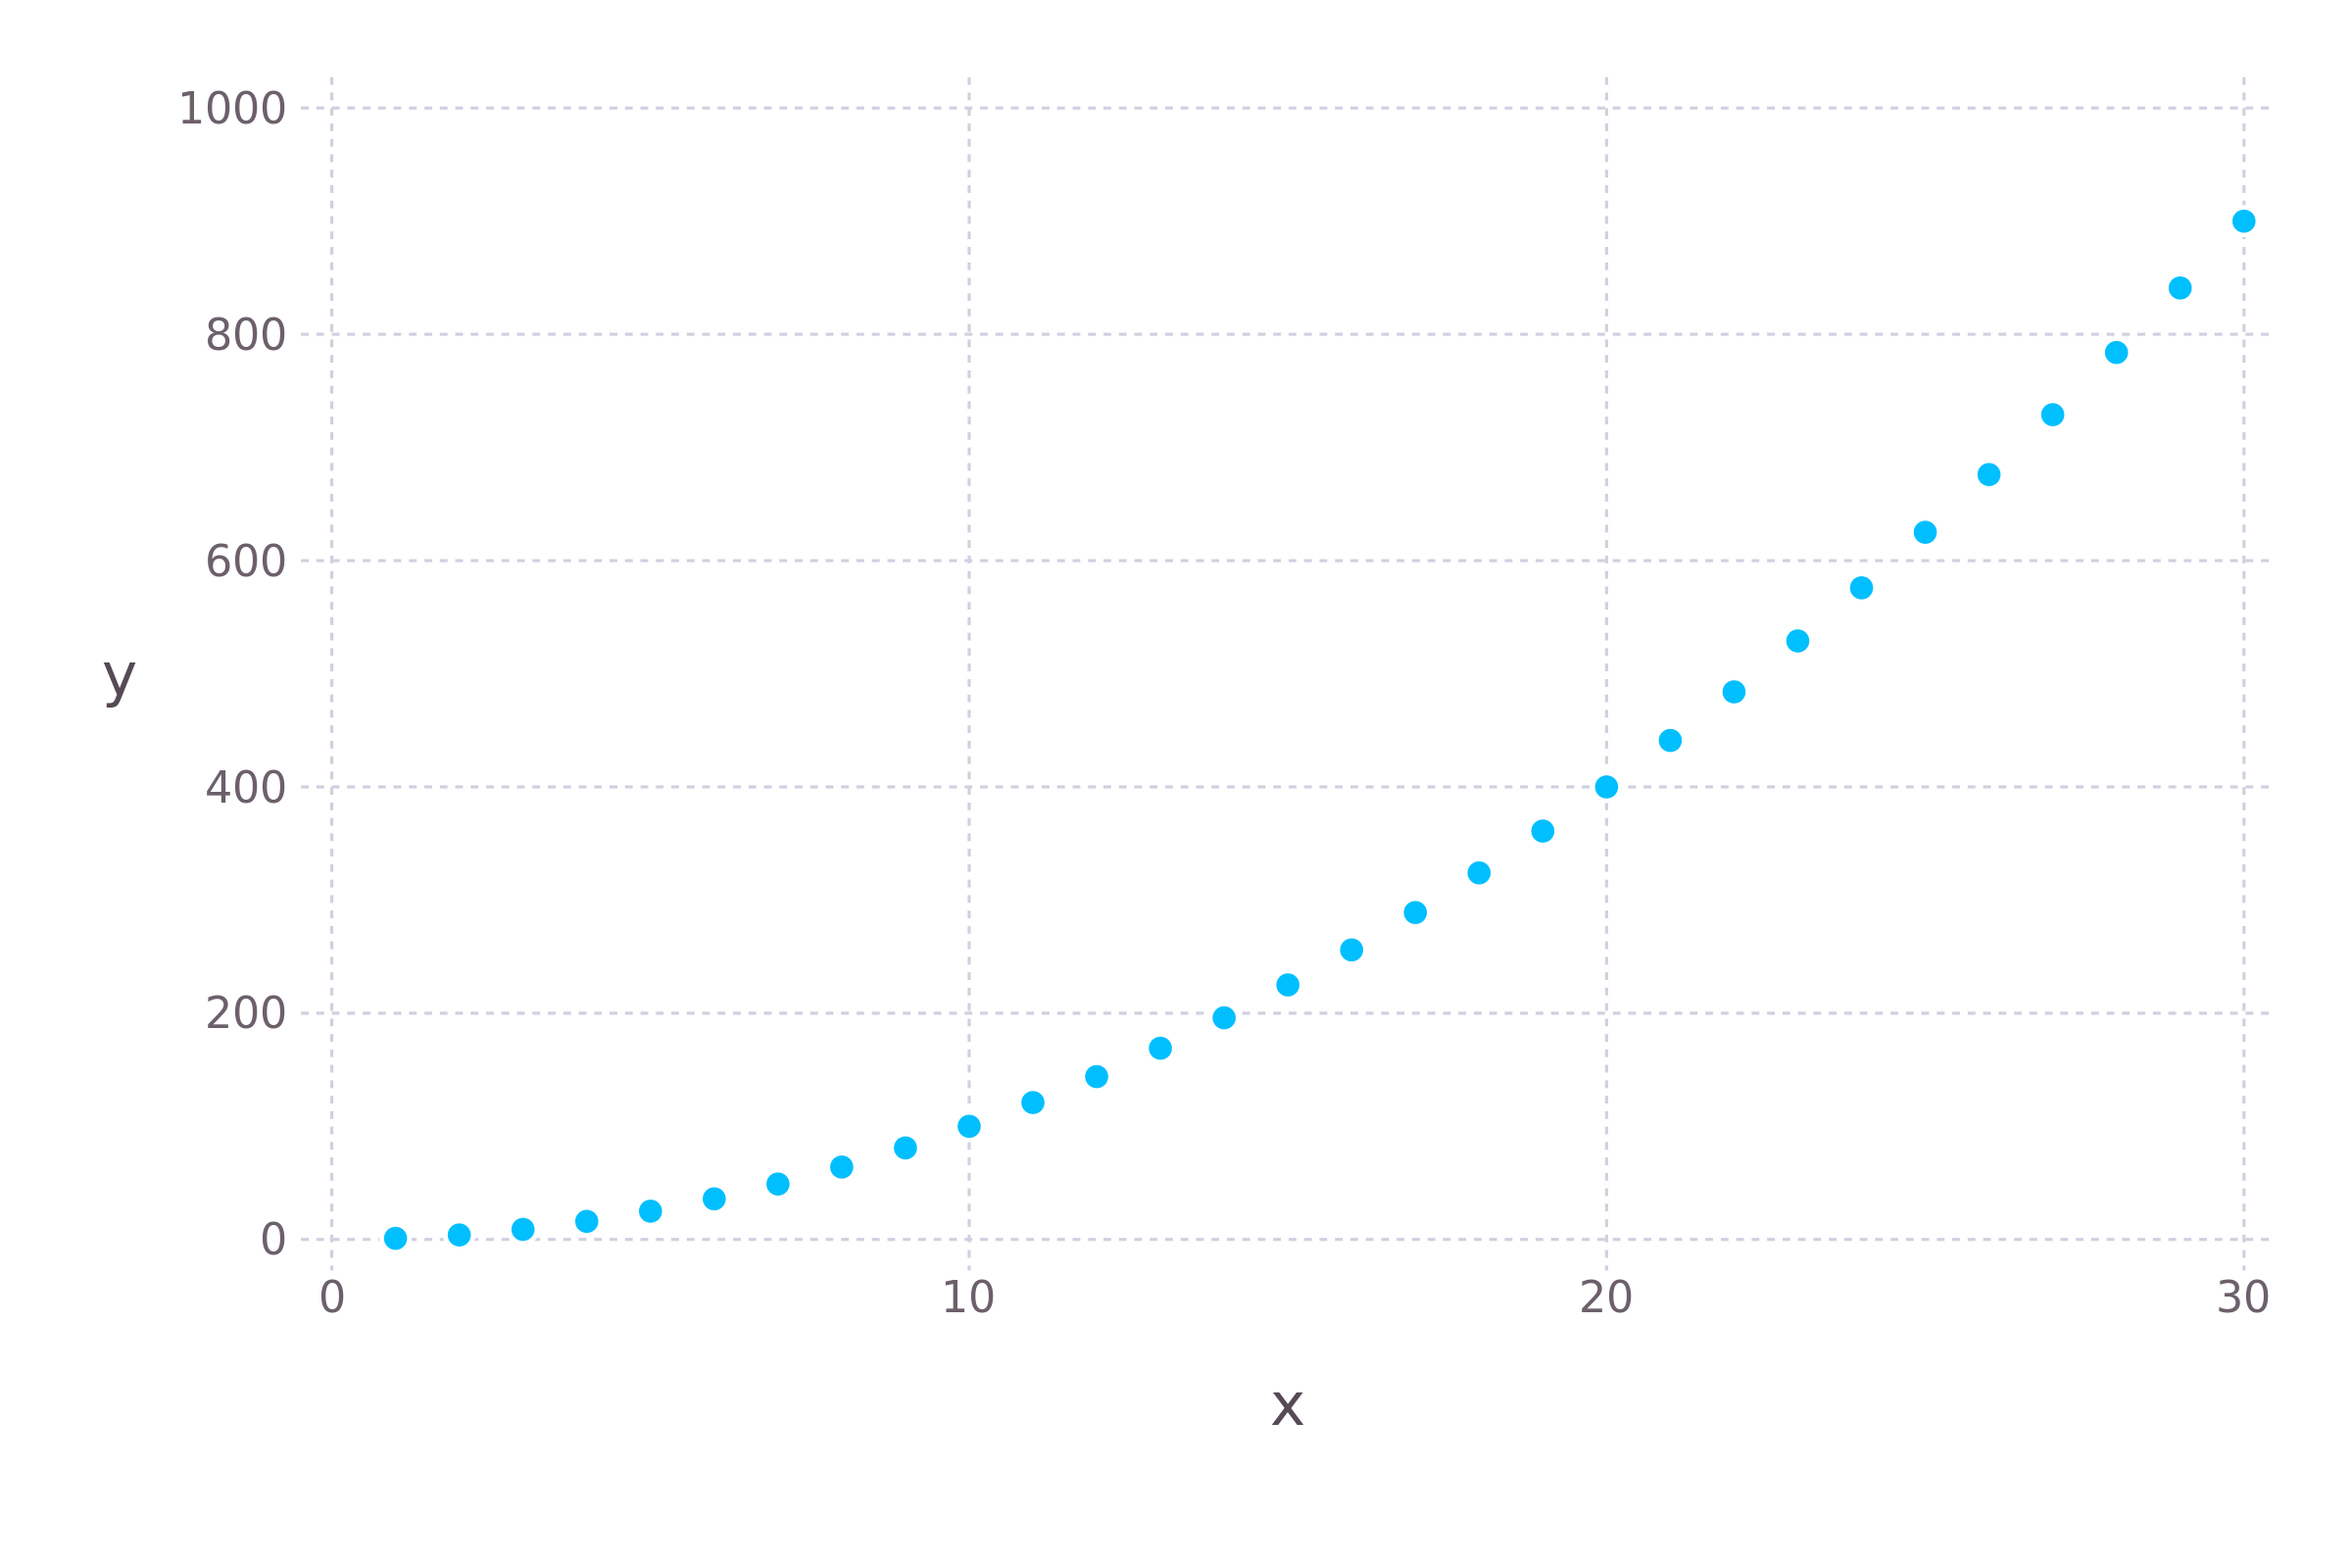
\includegraphics{build/im/example_plot.png}
\caption{Example plot.}\label{fig:example_plot}
}
\end{figure}

If the output is a string instead of the output you expected, then check
whether you load the related packages in time. For example, for this
Gadfly plot, you need to load Gadfly.jl together with Books.jl for
Requires.jl to work.

For multiple images, use
\passthrough{\lstinline!outputs(paths, objects)!}:

\begin{lstlisting}
function multiple_example_plots()
    paths = ["example_plot_$i" for i in 2:3]
    X = 1:30
    objects = [
        plot(x = X, y = X),
        plot(x = X, y = X.^3)
    ]
    outputs(paths, objects)
end
\end{lstlisting}

Resulting in Figure~\ref{fig:example_plot_2} and
Figure~\ref{fig:example_plot_3}:

\begin{figure}
\hypertarget{fig:example_plot_2}{%
\centering
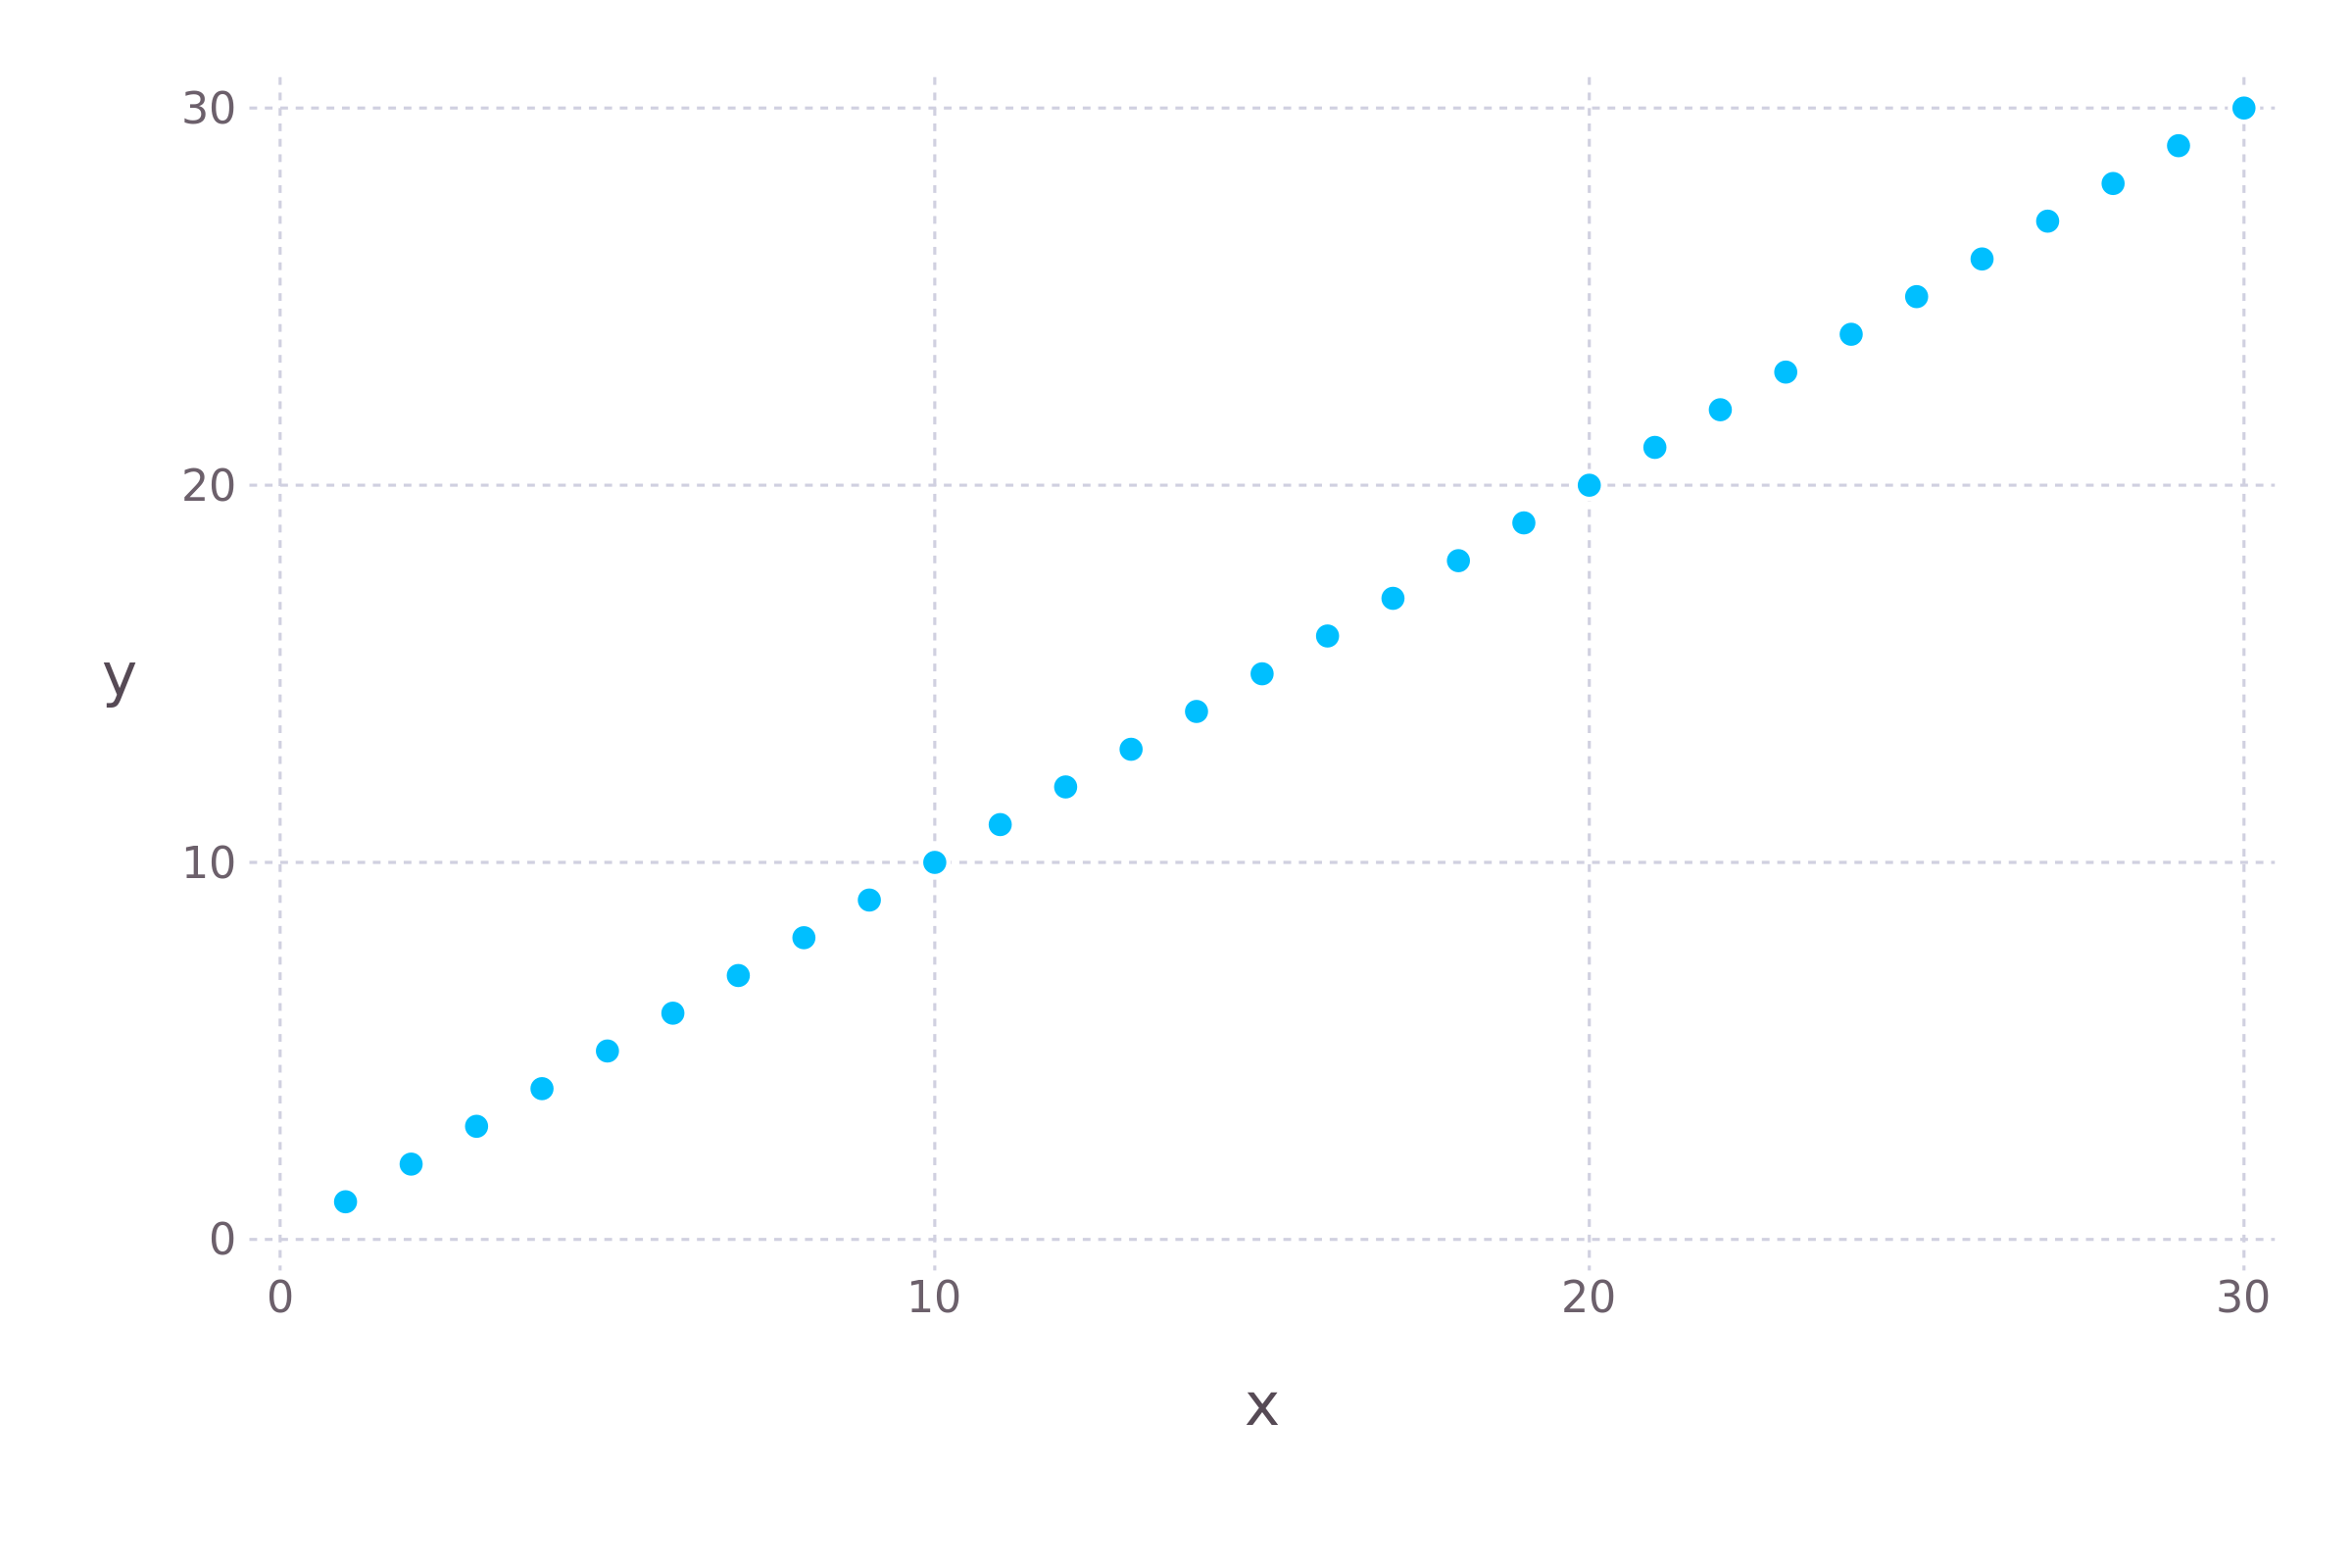
\includegraphics{build/im/example_plot_2.png}
\caption{Example plot 2.}\label{fig:example_plot_2}
}
\end{figure}

\begin{figure}
\hypertarget{fig:example_plot_3}{%
\centering
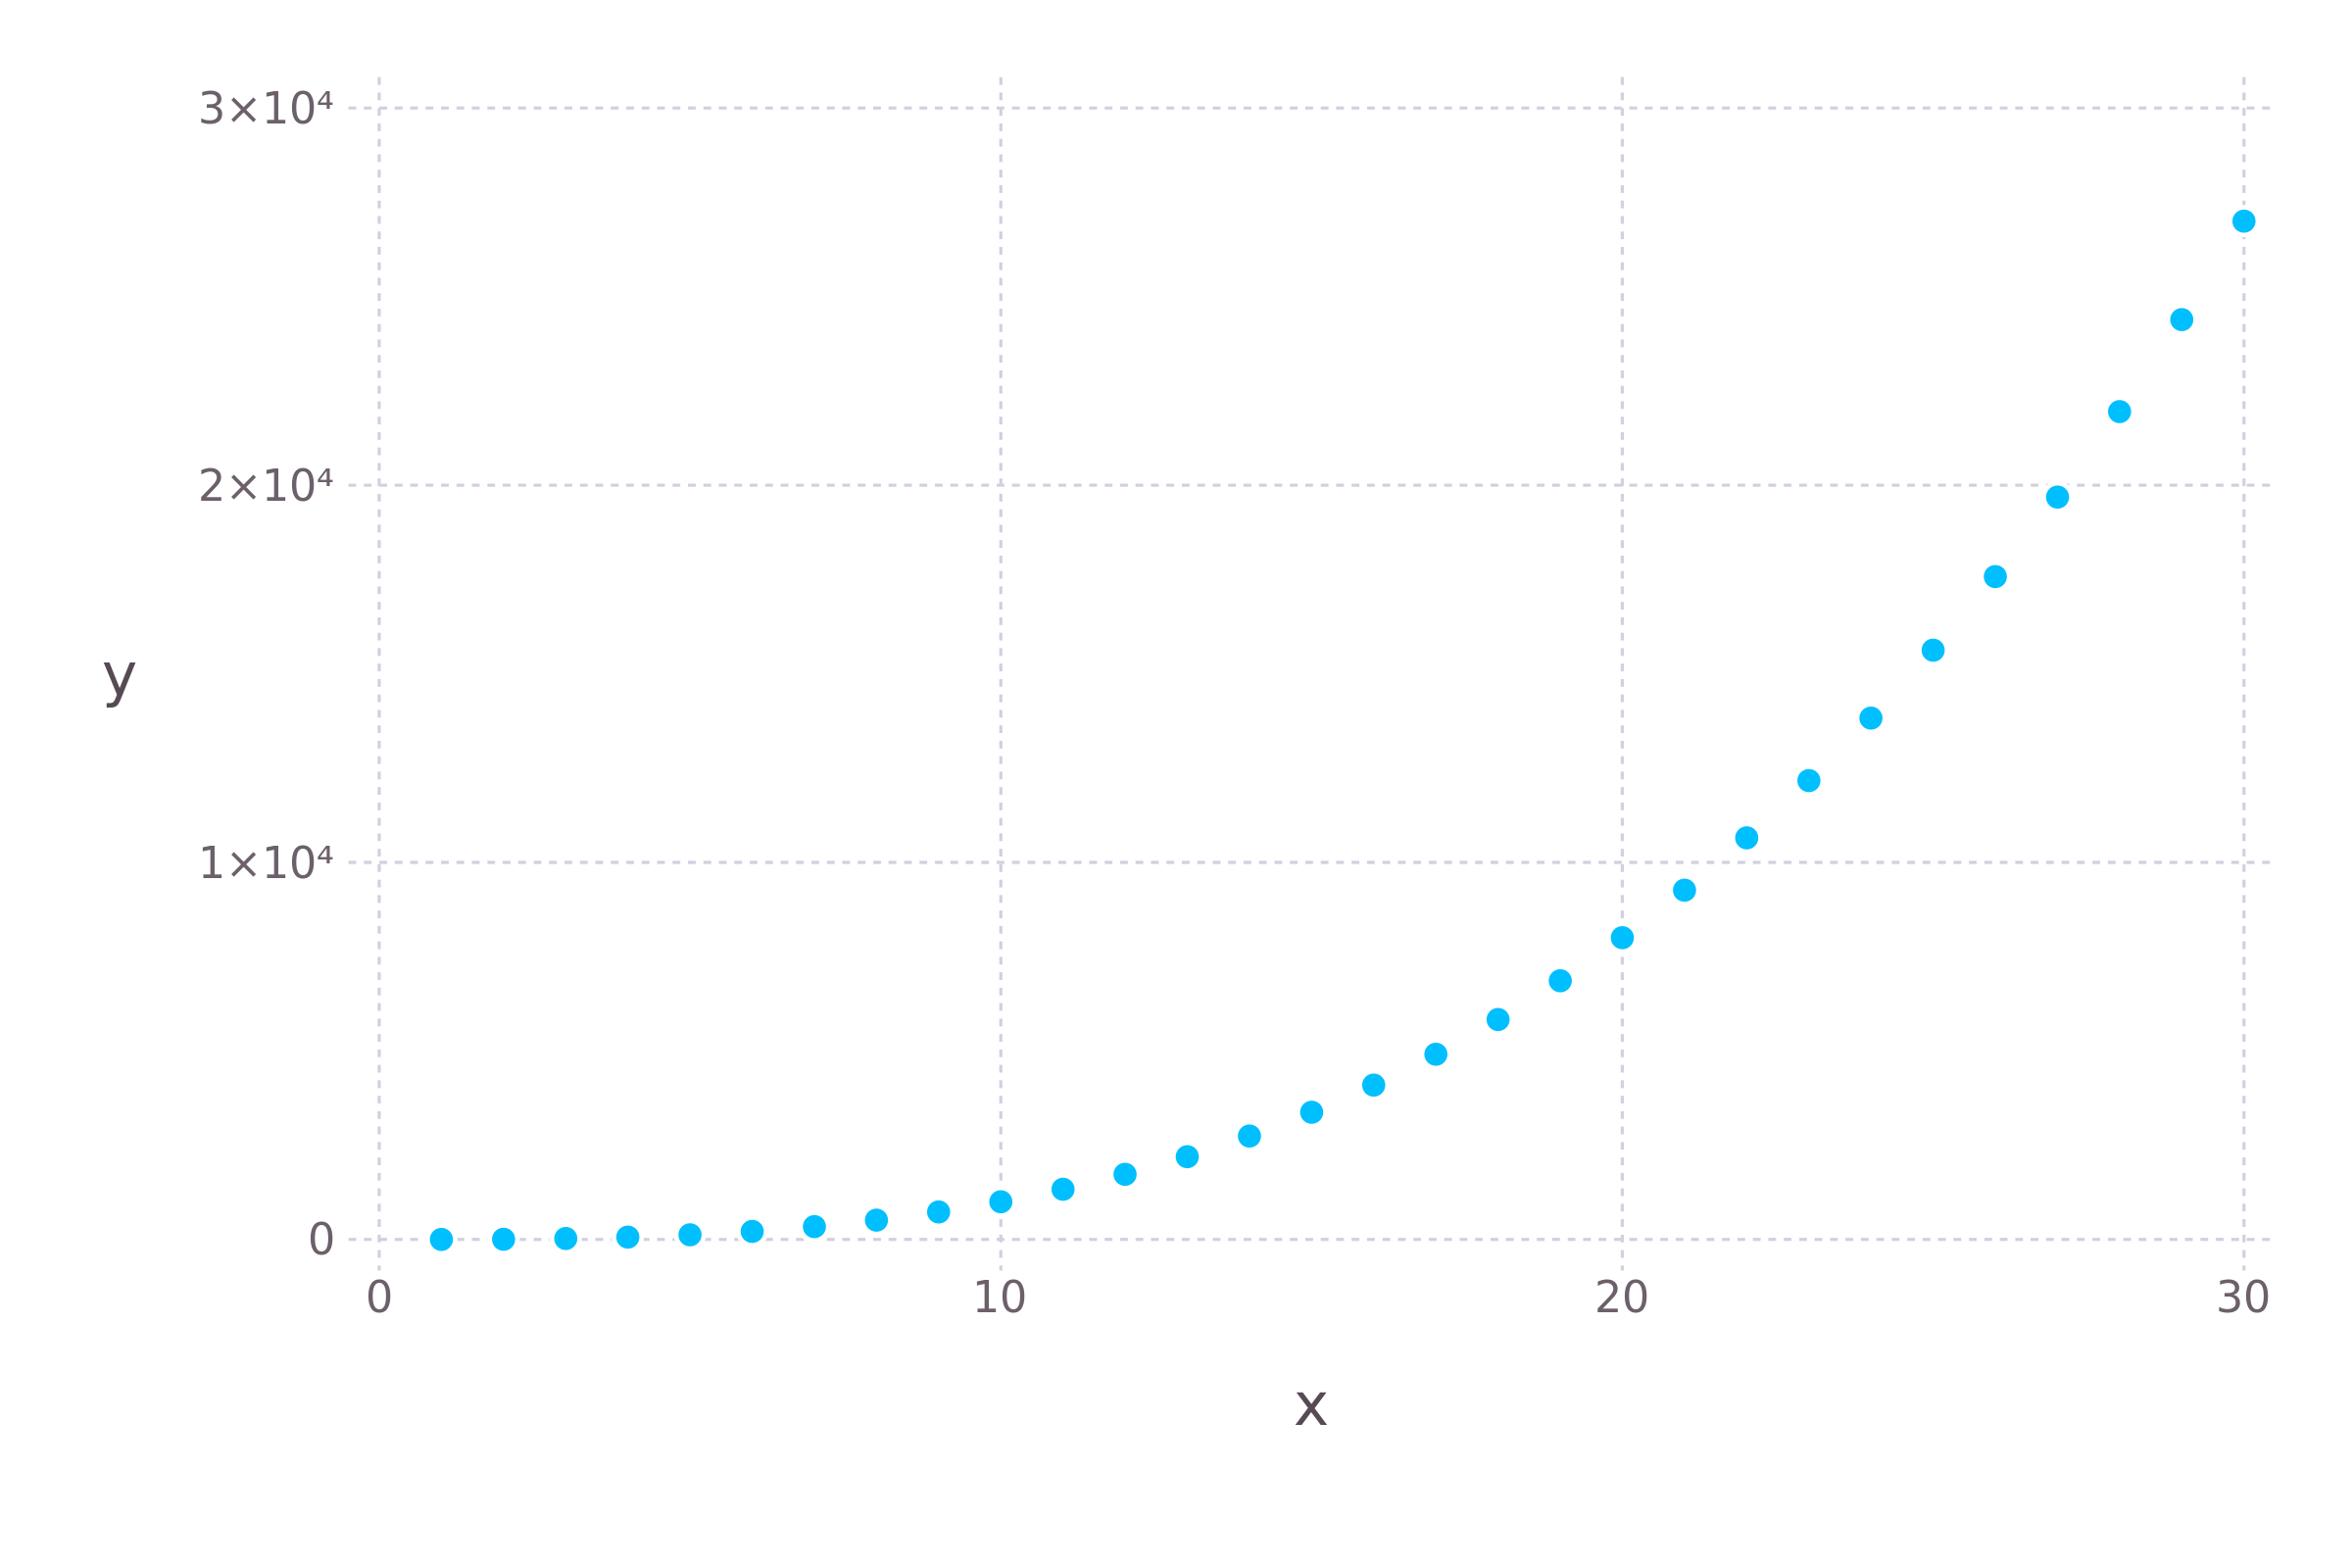
\includegraphics{build/im/example_plot_3.png}
\caption{Example plot 3.}\label{fig:example_plot_3}
}
\end{figure}

\hypertarget{other-notes}{%
\section{Other notes}\label{other-notes}}

\hypertarget{level-3-headings}{%
\subsection{Level 3 headings}\label{level-3-headings}}

These are hidden from the website menu.

\hypertarget{references}{%
\chapter*{References}\label{references}}
\addcontentsline{toc}{chapter}{References}

\hypertarget{refs}{}
\begin{cslreferences}
\leavevmode\hypertarget{ref-orwell1945animal}{}%
Orwell, G. (1945). \emph{Animal Farm: A Fairy Story}. Houghton Mifflin
Harcourt.
\end{cslreferences}

% \backmatter
\end{document}
